Over the last 20 years, the Internet of Things has developed and evolved continuously, from the beginning where it was the concept of using barcodes, and later RFID\cite{K.Ashton}, to track items in a warehouse, to today where our home appliances are filled with ``smart'' electronics, able to sense, react and notify the user of events, such as a notifying a user when the washing machine has finished a load of laundry, turn on a light when the user enters a room or adjust the heating schedule depending on who's home. Whilst the Internet of Things has been around for quite some time, under various guises, it's yet to become commercially successful and see wide-spread deployment; many believe that 2013 is the year that the Internet of Things will truly take off and become ubiquitous in our daily lives\cite{2013IoT}.

The rest of this section will discuss various different attempts made to create Internet of Things networks in the home.

\subsubsection{IoT protocol} % (fold)
\label{ssub:knot}
Our previous work\cite{KNoT} demonstrated the need for a new protocol specifically designed for constrained devices in the IoT paradigm, taking into consideration not only the computational constraints, but also the often limited power resources available. As a result, a lightweight and scalable networking protocol, tailored around the IoT architecture, was designed and implemented for TelosB motes running the Contiki OS. 

Within the protocol, devices in the IoT architecture were divided up into three categories of Things. Sensors, devices which sense the environment and transmit the data to interested parties at set intervals; actuators, devices which could receive commands and interact with the environment e.g. display data, turn on a light bulb; and controllers, one or more devices which controlled the network of things, connecting to both sensors and actuators to create a closed loop of control e.g. several sensors send temperature readings to a controller, which decides it's too hot and sends a command to the air conditioner actuator to cool the room. 

Whilst the protocol was deemed successful when compared to existing protocols, there are some issues. Firstly, there's no security, packets are transmitted in plain sight with no encryption. Secondly, in relation to integration, whilst the protocol worked well within the network of Things, it lacked integration into other, more powerful platforms, such as a PC, which would enable it to become far more powerful, dynamic and customisable, as well as allow users to interact with it more easily. 
% subsubsection knot (end)

\subsubsection{Smart Things} % (fold)
\label{ssub:smart_things}
Launched in 2012, the SmartThings platform aims to allow the user to turn any ordinary object in the home into a ``Smart'' object by giving it the ability to connect to the Internet. The platform consists of a central hub connected to the Internet, containing a low-power Zigbee radio, from which it connects to an array of SmartThings accessories as well as many pre-existing third party Zigbee devices. Some of these accessories include motion detectors, moisture sensors, vibration detectors, power-plug switches as well as many others. The user can then view and interact with their Smart Things through a cloud service via an Internet-connected PC or a smartphone, allowing them to either control the devices directly or set-up rules/schedules for devices.

\begin{figure}[h!]
\centering
    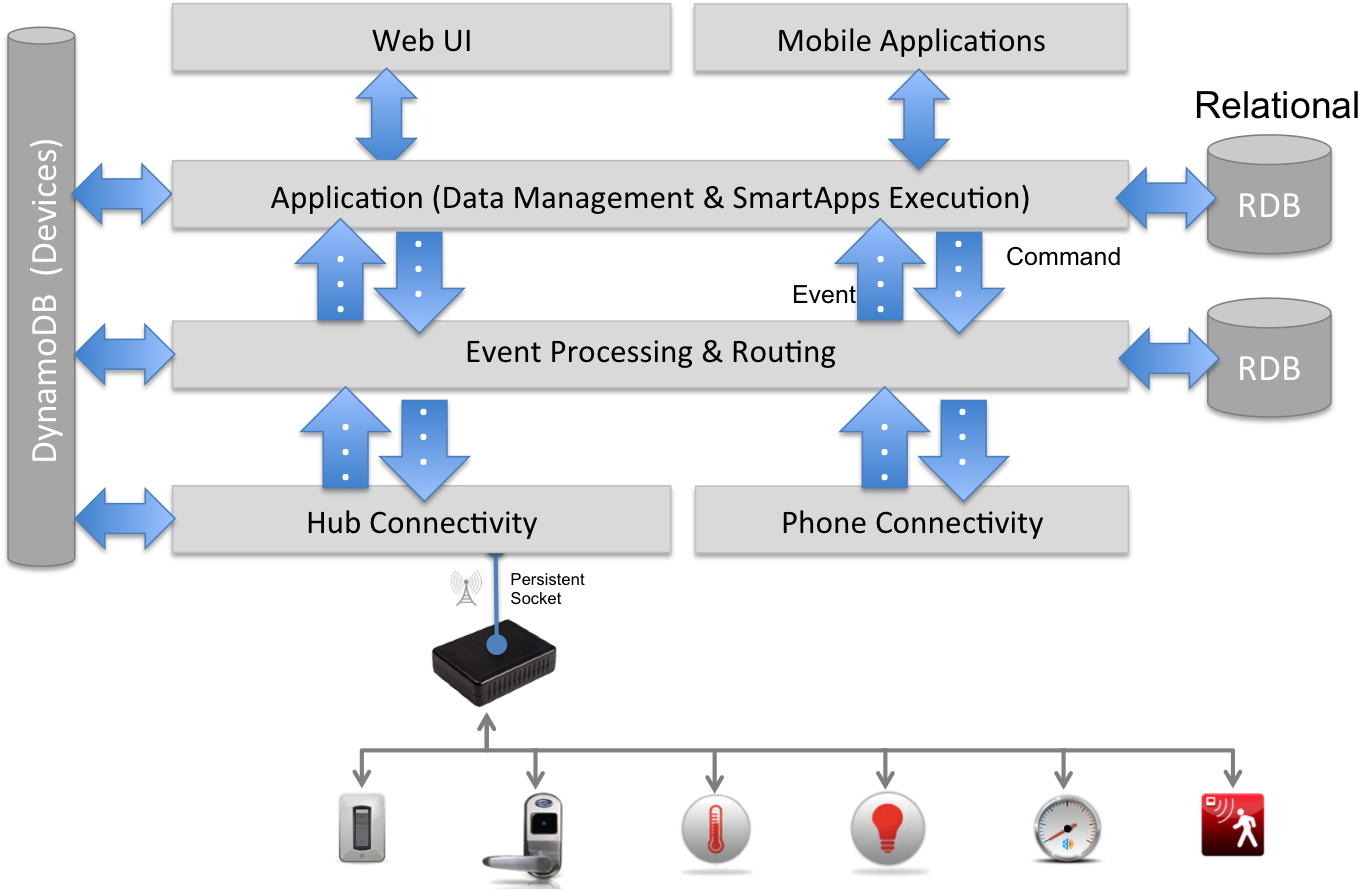
\includegraphics[scale=0.4]{images/smartThingsCloudFirstDiagram.png}
    \caption[]{Smart Things - Cloud approach\footnotemark}
    \label{fig:cloud}
\end{figure}
\footnotetext{Image from Smart Things developer support: \url{https://support.smartthings.com/entries/21603009-Device-Types-Capabilities-Attributes}}

As shown in figure \ref{fig:cloud}, Smart Things takes a cloud approach, offloading all processing to the cloud, leaving the hub to just act as a gateway and translator between the Things and the cloud. By utilising the cloud in this way, it enables the hub to be a very simple and low-power device, reducing both the acquisition and running costs for the user. It also allows the user to access their network of Things from anywhere, at any time, which would otherwise be difficult to do in a local approach. 

However, the cloud approach also has several drawbacks. By offloading the entire processing needs of the network, as shown above, the network of Things becomes vulnerable to failure if either the network fails or is unresponsive, or if the cloud service fails or goes down for maintenance. Another issue is the privacy of the user's data; how safe is the data in the cloud and how secure are the services they make available for users to interact with their devices? There have been many examples of online services that have been attacked, leaking user data and/or shutting down for extended periods of time \cite{Playstation, Amazon, Google}.
% subsubsection smart_things (end)

\subsubsection{CoAP} % (fold)
\label{ssub:core_coap}
CoAP, Constrained Application Protocol\cite{IETF_COAP_HTTP}, is currently a proposed IETF standard to create a request-response style web protocol, specifically designed to directly bridge the gap between the Internet and constrained devices, allowing Things to communicate and respond directly to other devices on the Internet, similar to the typical client-server interactions at present. The protocol is designed as an asynchronous RESTful protocol, to run on top of UDP, using a subset of the standard commands e.g., GET, PUT, DELETE. The reason is that due to the common commands, it allows for an easy transition to standard HTTP, if necessary, whilst reducing the complexity of the protocol.

Unlike the two platforms/protocols previously discussed, this protocol potentially places Things directly on the Internet just like normal HTTP servers. This not only makes these devices much easier to connect, as it's just like connecting to typical servers, but also has similar risks to Smart Things, where devices could be vulnerable and attacked directly, just like a typical server. In relation to this, Symantec recently discovered a new Linux worm\cite{IoTWorm} targeted directly at IoT devices, thus proving the possible risks of creating such devices.




% subsubsection core_coap (end)
